% Single file version of the paper. Paste it into a new Overleaf project and compile with pdfLaTeX.
% No other files are needed: tables, figures (pgfplots) and references are all inside this file.
\documentclass[10pt,conference]{IEEEtran}
\IEEEoverridecommandlockouts
\usepackage[T1]{fontenc}
\usepackage{cite}
\usepackage{amsmath,amssymb}
\usepackage{array}
\usepackage{booktabs}
\usepackage{xcolor}
\usepackage{pgfplots}
\pgfplotsset{compat=1.17}
\usepackage[hidelinks]{hyperref}

\newcolumntype{L}[1]{>{\raggedright\arraybackslash}p{#1}}

\begin{document}

\title{Noise drift of simulator trained quantum classifiers on IBM Heron processors}

\author{\IEEEauthorblockN{Pankaj Baid, Kartikey Gupta and Shreshtha Gupta}
\IEEEauthorblockA{Newton School of Technology, Rishihood University\\
Sonipat, Haryana, India\\
pankaj.baid2024@nst.rishihood.edu.in}}

\maketitle

\begin{abstract}
Quantum machine learning models are usually trained in noiseless simulation and then deployed on
hardware whose noise differs from the simulator and changes over time. We measured the effect of
this transition on three small quantum classifiers trained on two datasets. The frozen models were
run on two IBM Heron r2 processors in five sessions per device over 16 days, following an analysis
plan registered before the first session. The study used 227 seconds of free plan QPU time: 205
seconds for the campaign and 22 seconds for crosstalk pilots. Hardware accuracy was on average 9.2
points below the simulator. An emulator built from the reported calibration data overestimated
hardware accuracy by 5.5 points but ranked the configurations well ($r=0.87$). Between sessions
the variance of the measured features was 3.8 times the variance expected from shot noise, on both
devices. The noise acted mainly as a small and stable contraction of the features. No low cost
repair recovered more than 15\% of the accuracy gap, and only readout correction measured in the
same job and a classifier head trained on emulated noisy features gave clear gains. Conformal
prediction sets calibrated in simulation undercovered on hardware, while sets calibrated on
hardware data reached the nominal coverage. Code and data are public.
\end{abstract}

\begin{IEEEkeywords}
quantum machine learning, noise drift, error mitigation, conformal prediction, IBM quantum
\end{IEEEkeywords}

%======================================================================
\section{Introduction}

Most quantum classifiers are developed and trained in simulation, where computation is free, fast
and noiseless. Real processors are not. Gate errors, readout errors and decoherence distort the
expectation values that a classifier reads out \cite{wang2021nibp,heyraud2022noisykernels}. The error rates also change between calibrations \cite{realtimecal2023}. A model evaluated on one
day may therefore perform differently a few days later or on another processor of the same type.

Earlier work has measured this gap mainly at a single point in time. QuantumNAT showed that
noise acts on the outputs roughly as a scale and a shift \cite{wang2022quantumnat}. Readout
mitigation removes the bias that measurement errors add \cite{nation2021m3,vandenberg2022trex}.
On the uncertainty side, conformal prediction can wrap the output of a quantum model in a set of
labels with a coverage guarantee \cite{park2023qcp}. An adaptive version keeps that guarantee when
the noise moves, though it was tested on data from one day \cite{spencer2026aqcp}. Closest to our
work, a QAOA study on three Heron processors found that emulators built from calibration data were
too optimistic \cite{qaoa2026drift}.

We did not find a study that returns the same frozen classifiers to hardware repeatedly, on more
than one device, and tests whether the observed changes exceed shot noise. The cost of each
correction is also rarely reported. This cost matters in practice: IBM's free Open Plan provides
ten minutes of QPU time every 28 days, so every additional calibration circuit reduces the budget
left for the experiment.

This paper reports such a study. We trained three small classifiers on two datasets in simulation
and froze them. We then ran the same 182 inputs per dataset on two IBM Heron r2 processors,
\texttt{ibm\_fez} and \texttt{ibm\_kingston}, five sessions on each over 16 days. To fit the budget we placed 14 copies of every four qubit circuit side by side on the chip, which
reduced one session to about 20 seconds of QPU time. The hypotheses and the analysis plan were
registered as a git tag before the first session, so that the decision rules could not be adjusted
after seeing the data. We address four research questions.

\begin{itemize}
\item \textbf{RQ1} How large is the accuracy gap between simulator and hardware, and can an emulator
predict it?
\item \textbf{RQ2} How much do results change between sessions and devices beyond shot noise, and
which calibration numbers explain the change?
\item \textbf{RQ3} Does the simple scale and shift picture of the noise hold on Heron, and does it
stay stable over time?
\item \textbf{RQ4} Which low cost repairs restore accuracy and reliable uncertainty, and what does
each one cost in QPU seconds?
\end{itemize}

The contributions are a registered and budget safe protocol for tracking quantum
classifiers on cloud hardware, paired measurements on two devices that answer these questions, a
comparison of repairs and prediction set methods by their QPU cost, and the full code and raw data.

We do not claim quantum advantage. In the simulator a tuned RBF support vector
machine beats all three quantum models on two curves (0.987 against 0.927), and on breast cancer
the differences lie within the confidence intervals (Table~\ref{tab:sim}). Larger benchmark studies found the same
\cite{bowles2024benchmarking,schuld2022advantage}. Our question is narrower: how reliably a given quantum model behaves once it leaves the
simulator.

%======================================================================
\section{Related work}

\subsection{Quantum classifiers}
The first hardware demonstrations of quantum classification used a variational circuit and a
quantum kernel on a superconducting chip \cite{havlicek2019supervised}. Since then a few model
families have become common. Circuits that load the input several times can act as universal
classifiers \cite{perezsalinas2020reuploading}. Projected models measure simple local quantities
and hand them to a classical learner \cite{huang2021power}. Reservoir style models keep a fixed
random circuit and train only the readout \cite{yasuda2023qrc}. We picked one model from each of
these families.

\subsection{Noise and its correction}
Noise affects quantum models in several ways. It can flatten the gradients of deep variational
circuits \cite{wang2021nibp}, it can push kernel values toward a constant
\cite{thanasilp2024concentration}, and it limits what a noisy kernel is able to learn at all
\cite{heyraud2022noisykernels}. QuantumNAT addressed this with normalisation and noise injection
during training and reported gains of up to 43\% on older IBM devices \cite{wang2022quantumnat}.
The QuantumNAS authors noted that a circuit has to be tested right after it is
designed, because the noise drifts \cite{wang2022quantumnas}. Error mitigation works after the run.
Readout mitigation \cite{nation2021m3} and zero noise extrapolation \cite{temme2017zne} are the
usual examples, and learned mitigation reduces its cost, although its authors list drift as
an open problem \cite{liao2024mlqem}. Most of these methods need extra circuits. On a free budget
that is a real cost, so we only tested repairs that need few circuits or none.

\subsection{Uncertainty}
A classifier should also report how confident it is. The expected calibration error checks
whether predicted probabilities match the observed frequency of correct predictions
\cite{guo2017calibration}. Conformal prediction returns a set of labels that
should contain the true one with a chosen probability \cite{park2023qcp}. The guarantee assumes exchangeable data, an assumption that time varying hardware noise can
violate. Adaptive
conformal inference (ACI) relaxes this assumption by updating its miscoverage level online \cite{gibbs2021aci}, and AQCP
brought the idea to quantum models using one day of hardware data \cite{spencer2026aqcp}.

\subsection{Studies that follow hardware over time}
Few studies return to the same workload on hardware over several days. The closest example we
found is a QAOA study on three Heron processors that repeated its circuits 9 to 12 days later.
It concluded that calibration data help to pick good qubits, but an emulator built from them
overstated the gain on real hardware \cite{qaoa2026drift}. QBioBench tested quantum classifiers on
a single IBM processor and showed that small test sets give unstable accuracy \cite{qbiobench2026}.
Another group moved a learned noise model from one IBM device to another
\cite{farib2026crossdevice}. Running many small circuits side by side saves time but can add crosstalk between them
\cite{murali2020crosstalk,ohkura2022simultaneous}, which we checked with a pilot before the
campaign.

\begin{table*}[t]
\centering
\caption{Closest earlier studies and what they leave open.}
\label{tab:related}
\footnotesize
\renewcommand{\arraystretch}{1.15}
\begin{tabular}{L{2.6cm}L{3.8cm}L{4.0cm}L{5.6cm}}
\toprule
Study & What was studied & Hardware and time & What is left open \\
\midrule
QuantumNAT \cite{wang2022quantumnat} & quantum neural networks on 8 tasks & 6 IBM devices & change across days not reported \\
AQCP \cite{spencer2026aqcp} & adaptive conformal prediction & one IBM device on one day & several days left for future work \\
QAOA drift study \cite{qaoa2026drift} & QAOA for MaxCut & 3 Heron r2 devices with repeats after 9 to 12 days & optimisation and not classification \\
QBioBench \cite{qbiobench2026} & biosignal classifiers & one IBM Nighthawk device & one device and small test sets \\
Cross device transfer \cite{farib2026crossdevice} & noise models of circuit outputs & \texttt{ibm\_fez} and \texttt{ibm\_marrakesh} & output distributions and not classifier accuracy \\
\midrule
\textbf{This study} & three classifiers on two datasets & 2 Heron r2 devices with 10 sessions over 16 days & small frozen models on a free plan \\
\bottomrule
\end{tabular}
\end{table*}

\subsection{Research gap}
Table~\ref{tab:related} puts the closest studies side by side. The evidence on how deployed
classifiers change over days is thin. Corrections are mostly tested on one device, their cost is
rarely measured, and small test sets make any single session unreliable. To our knowledge no
earlier study repeats frozen quantum classifiers on more than one Heron processor over several
days while also separating drift from shot noise, pricing each repair in QPU time and checking
conformal coverage on the same data.

%======================================================================
\section{Problem statement}

We consider a classifier that is trained in a noiseless simulator and then frozen. We ask three
questions. How much do its accuracy and the reliability of its predictions
change when it runs on real processors on different days? How much of that change is real drift
and not just shot noise? And which cheap repairs win back the loss for the least QPU time?

\subsection{Setting}
An input $x$ has $n=4$ features scaled to $[0,\pi]$. A fixed circuit prepares a state
$\rho_\theta(x)$ on four qubits. The model measures Pauli expectation values and feeds them to a
logistic head:
\begin{align}
\hat p(y=1\mid x)&=\sigma\!\Big(w^\top\frac{\phi(x)-\mu}{s}+b\Big), \label{eq:model}\\
\phi_j(x)&=\operatorname{tr}\!\big[P_j\,\rho_\theta(x)\big]. \nonumber
\end{align}
Here $\sigma$ is the logistic function, $P_j$ is a Pauli string, and $\mu$ and $s$ are the mean and standard deviation of the training features, applied element wise. All parameters are fixed after training. On hardware each circuit runs
with $N=500$ shots, where a shot is one run of the circuit followed by one measurement. Because the number of shots is finite, each estimated feature carries a sampling error, called
shot noise, with variance $(1-\phi_j^2)/N$.

\subsection{What we measure}
\begin{itemize}
\item \emph{Gap and emulator error.} The gap is simulator accuracy minus hardware accuracy. The
emulator error is emulated accuracy minus hardware accuracy, where the emulator is a noisy
simulation that uses the calibration data IBM publishes for the device.
\item \emph{Drift.} For each input and feature we divide the variance across sessions by the
variance that shot noise alone would produce:
\begin{equation}
r(x,j)=\frac{\operatorname{Var}_t\big[\hat\phi_{t,j}(x)\big]}
{\operatorname{E}_t\big[(1-\hat\phi_{t,j}(x)^{2})/N\big]}.
\label{eq:drift}
\end{equation}
Under shot noise alone the expected ratio is one. A mean ratio whose 95\% bootstrap interval lies
well above one indicates variation between sessions beyond the estimated shot noise. This reading
assumes that the shot noise variance is estimated correctly and that sessions are independent.
\item \emph{Noise map.} The scale $\gamma$ and shift $\beta$ in
$\phi_{\mathrm{hw}}\approx\gamma\,\phi_{\mathrm{sim}}+\beta$, and how much they move.
\item \emph{Repairs.} How much accuracy each repair adds and how many extra QPU seconds it needs.
\item \emph{Uncertainty.} Prediction sets with a nominal coverage of 0.90. We report the empirical coverage, its worst case
and the mean set size.
\end{itemize}

\subsection{Hypotheses}
Before the first campaign session we registered five hypotheses, each with a fixed decision rule
based on a 95\% bootstrap interval (git tag \texttt{prereg-v1}, 27 October 2026).
Table~\ref{tab:hypotheses} lists them with the results.

\subsection{Scope}
We capped the campaign at 400 seconds of QPU time. The models are small, with four qubits and two
datasets, and we never train on hardware. This is a measurement of how models behave on two
processors of one family. It is not a general theory of quantum noise.

%======================================================================
\section{Methodology}

\subsection{Datasets}
Both tasks are binary with four features. \emph{Two curves} comes from the benchmark suite of
Bowles et al.~\cite{bowles2024benchmarking}. The two classes lie on the same curve, one slightly
shifted from the other. \emph{Breast cancer} is the Wisconsin diagnostic dataset
\cite{wolberg1993breast}, reduced to four principal components. Each dataset gets 240 training
inputs, 100 validation inputs, a labelled pool of 32 inputs that we use only on hardware, and a
fixed test set of 150 inputs. The same 182 hardware inputs run in every session.

\subsection{Models}
All three models measure Pauli features on four qubits and pass them to the head in
Eq.~\eqref{eq:model}.
\begin{itemize}
\item \textbf{M1} is a data reuploading classifier \cite{perezsalinas2020reuploading} with three
layers and 28 trained circuit parameters. It reads four $\langle Z\rangle$ values.
\item \textbf{M2} uses projected features \cite{huang2021power}. A single fixed encoding layer is
measured in the X, Y and Z bases, which gives 12 features.
\item \textbf{M3} is a quantum extreme learning machine, related to quantum reservoir computing
\cite{yasuda2023qrc}. Two fixed random layers give 10 features.
\end{itemize}
Each head is fitted on exact simulator features with five fold cross validation. For reference we also tuned three classical models on the same inputs: logistic regression, an
RBF support vector machine and a small neural network (Table~\ref{tab:sim}).

\begin{table}[t]
\centering
\caption{Test accuracy in the noiseless simulator for the quantum models and the tuned classical
models. With 150 test inputs one accuracy value is uncertain by about $\pm$5 points.}
\label{tab:sim}
\footnotesize
\begin{tabular}{lcc}
\toprule
Model & Two curves & Breast cancer \\
\midrule
M1 reuploading & 0.927 & 0.967 \\
M2 projected & 0.873 & 0.933 \\
M3 extreme learning & 0.847 & 0.913 \\
\midrule
Logistic regression & 0.733 & 0.940 \\
RBF support vector machine & 0.987 & 0.940 \\
Small neural network & 0.973 & 0.960 \\
\bottomrule
\end{tabular}
\end{table}

\subsection{Hardware protocol}
We used two 156 qubit IBM Heron r2 processors through the free Open Plan and the Qiskit Runtime
sampler \cite{javadiabhari2024qiskit}. Our first choice for the second device was
\texttt{ibm\_marrakesh}. During the pilot it went into maintenance with more than two thousand jobs
waiting, so we cancelled our job there (at no cost) and switched to \texttt{ibm\_kingston}
before freezing the plan.

One session is one job. It contains a circuit block for each dataset, model and measurement basis,
plus two readout calibration circuits. Model circuits use 500 shots. We switched off twirling and dynamical decoupling in order to measure the raw device noise.

Packing kept the cost within the budget. Fourteen copies of each circuit run side by side on separate
chains of four qubits, with at least one idle qubit between neighbours. We chose the chains once
from the calibration data and kept them fixed for the whole campaign. Input $i$ always runs on
chain $i \bmod 14$, so every input meets the same qubits in every session. Before the campaign we ran a pilot with 28 inputs per device, once packed and once with each circuit alone. Every
difference between the two had an interval that included zero, so packing caused no detectable change. At this sample size the pilot can only exclude large
crosstalk effects.

Each device ran five sessions. The budget meter estimated 33 seconds per session including a
safety margin, and the billed time was 20 or 21 seconds. In total the ten sessions used 205 seconds
and the two pilots 22 seconds, which gives the 227 seconds reported in the abstract. Queue waits
were mostly short; the longest, for the \texttt{ibm\_kingston} pilot, was almost five hours. For every session we saved the raw counts
and the calibration data both at submission and at job start. The budget meter refused
any job that would push us past the cap.

\subsection{Emulator and repairs}
Before each job an emulator predicts the result. It is a Qiskit Aer simulation with a noise model
built from the calibration data of that moment. It simulates one chain at a time, so it contains no crosstalk. All repairs are computed afterwards from the same hardware counts.
\begin{itemize}
\item \textbf{R0} uses the simulator head as it is. This is the baseline.
\item \textbf{R1} rescales each feature with the mean and spread of the batch being scored, the
normalisation step of QuantumNAT \cite{wang2022quantumnat}.
\item \textbf{R2$_k$} refits the head on the first $k$ labelled pool inputs of the session, with
$k$ equal to 8, 16 or 32. A penalty keeps the new head close to the simulator head.
R2$_{16}^{\mathrm{s1}}$ reuses the labels from session 1 in all later sessions.
\item \textbf{R3} undoes readout errors with a confusion matrix for each qubit
\cite{nation2021m3}. R3$_\mathrm{m}$ measures these matrices inside the same job, while
R3$_\mathrm{r}$ takes them from IBM's published calibration.
\item \textbf{R4} trains the head on training inputs that were passed through the emulator first.
The head is thus fitted to noisy features before it is used on hardware.
\end{itemize}
Each repair is charged for its extra shots: R2$_k$ for its $k$ labelled inputs and R3$_\mathrm{m}$
for its two calibration circuits. R1, R3$_\mathrm{r}$ and R4 need no extra QPU time.

\subsection{Prediction sets}
We use split conformal prediction with a nominal coverage of 0.90 \cite{park2023qcp} and try three
calibration sets. CP$_\mathrm{sim}$ is calibrated on simulator data, CP$_\mathrm{s1}$ on the
hardware pool of session 1 and CP$_\mathrm{same}$ on the pool of the same session. ACI
\cite{gibbs2021aci} starts from simulator data and updates its miscoverage level after each test label is revealed. We also report the expected calibration error \cite{guo2017calibration}.

\subsection{Statistics}
Drift is tested with Eq.~\eqref{eq:drift}. To identify which calibration quantities are associated with the error, we regress the feature error of each input on four properties of its chain: readout error,
CZ error, $T_1$ and $T_2$. Every other interval is a bootstrap interval with 2000 resamples. We call
one combination of device, session, dataset and model a case, and there are 60 cases in all.

%======================================================================
\section{Results}

All 10 sessions were completed, five on each device.

\subsection{Simulator, emulator and hardware (RQ1)}
Without any repair, hardware accuracy was 9.2 points below the simulator on average
(Table~\ref{tab:accuracy}). The gap was positive in 55 of the 60 cases and ranged from $-1.3$ to
26.7 points. The gap depended mainly on the task: 14.6 points on two curves but only 3.8 on breast
cancer. M3 lost the most (11.9 points) and M1 the least (7.3). Between the devices,
\texttt{ibm\_fez} lost 8.0 points and \texttt{ibm\_kingston} 10.4.

The emulator systematically overestimated hardware accuracy. In 51 of 60 cases it predicted a
higher accuracy than the hardware achieved, by 5.5 points on average (interval 4.2 to 6.9), so H1 is supported. It nevertheless ranked the cases well. Emulated and hardware accuracy correlated with $r=0.87$ (Fig.~\ref{fig:emu}).
The slope of hardware on emulated accuracy was 1.31, so weaker configurations lost more on
hardware than the emulator predicted.

\begin{table}[t]
\centering
\caption{Mean test accuracy over all sessions and both devices. SIM is the simulator. EMU is the
emulator. R0 is hardware without repair. R3$_\mathrm{m}$ and R4 are the two best repairs.}
\label{tab:accuracy}
\footnotesize
\setlength{\tabcolsep}{4pt}
\begin{tabular}{llccccc}
\toprule
Dataset & Model & SIM & EMU & R0 & R3$_\mathrm{m}$ & R4 \\
\midrule
Breast cancer & M1 & 0.967 & 0.955 & 0.919 & 0.920 & 0.918 \\
Breast cancer & M2 & 0.933 & 0.915 & 0.921 & 0.925 & 0.925 \\
Breast cancer & M3 & 0.913 & 0.896 & 0.860 & 0.868 & 0.849 \\
Two curves & M1 & 0.927 & 0.903 & 0.829 & 0.841 & 0.825 \\
Two curves & M2 & 0.873 & 0.790 & 0.716 & 0.731 & 0.741 \\
Two curves & M3 & 0.847 & 0.781 & 0.663 & 0.683 & 0.701 \\
\bottomrule
\end{tabular}
\end{table}

\begin{figure}[t]
\centering
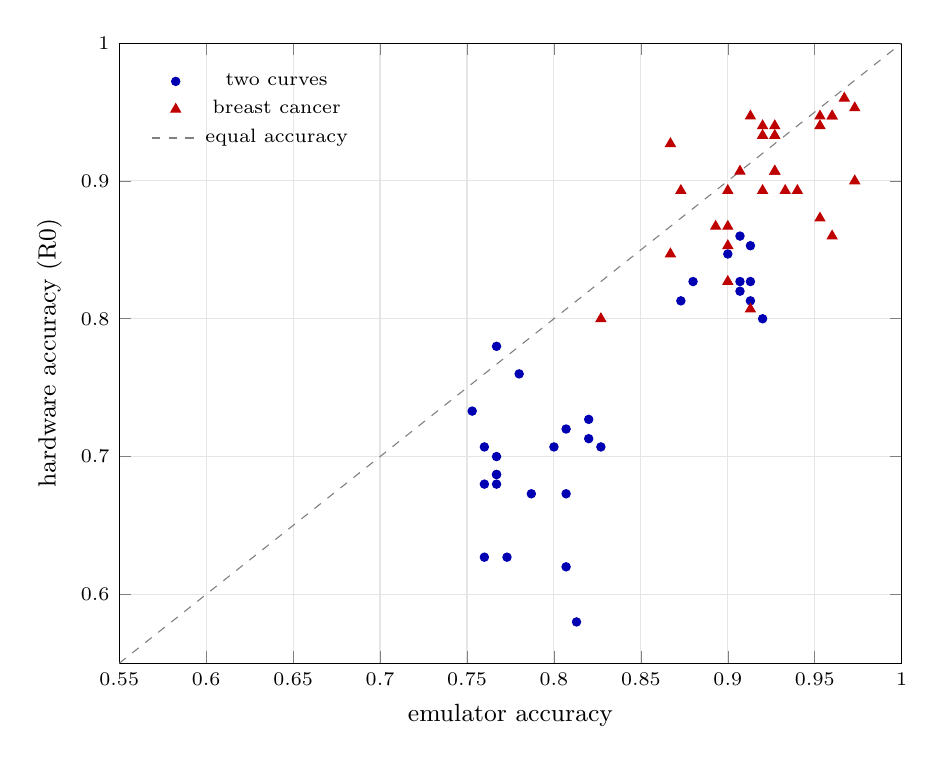
\begin{tikzpicture}
\begin{axis}[
  width=0.95\columnwidth, height=0.78\columnwidth,
  xmin=0.55, xmax=1.0, ymin=0.55, ymax=1.0,
  xlabel={emulator accuracy}, ylabel={hardware accuracy (R0)},
  tick label style={font=\scriptsize}, label style={font=\small},
  legend pos=north west, legend style={font=\scriptsize, draw=none, fill=none},
  grid=major, grid style={gray!20}]
\addplot[only marks, mark=*, mark size=1.5pt, color=blue!70!black] coordinates {
(0.920,0.800) (0.767,0.680) (0.787,0.673) (0.907,0.860) (0.827,0.707) (0.813,0.580)
(0.913,0.853) (0.780,0.760) (0.767,0.700) (0.900,0.847) (0.767,0.780) (0.773,0.627)
(0.880,0.827) (0.760,0.680) (0.760,0.707) (0.913,0.827) (0.753,0.733) (0.807,0.620)
(0.907,0.827) (0.807,0.673) (0.807,0.720) (0.873,0.813) (0.800,0.707) (0.767,0.687)
(0.913,0.813) (0.820,0.727) (0.767,0.687) (0.907,0.820) (0.820,0.713) (0.760,0.627)};
\addlegendentry{two curves}
\addplot[only marks, mark=triangle*, mark size=2pt, color=red!75!black] coordinates {
(0.973,0.900) (0.873,0.893) (0.867,0.847) (0.960,0.947) (0.920,0.940) (0.900,0.893)
(0.967,0.960) (0.913,0.947) (0.907,0.907) (0.973,0.953) (0.927,0.940) (0.920,0.893)
(0.960,0.947) (0.920,0.933) (0.927,0.907) (0.953,0.873) (0.940,0.893) (0.900,0.827)
(0.960,0.860) (0.927,0.933) (0.913,0.807) (0.893,0.867) (0.867,0.927) (0.827,0.800)
(0.953,0.940) (0.927,0.907) (0.900,0.867) (0.953,0.947) (0.933,0.893) (0.900,0.853)};
\addlegendentry{breast cancer}
\addplot[dashed, gray, domain=0.55:1.0] {x};
\addlegendentry{equal accuracy}
\end{axis}
\end{tikzpicture}
\caption{Emulator accuracy against hardware accuracy. Each point is one device, session, dataset
and model. Most points fall below the dashed line, so the emulator is too optimistic.}
\label{fig:emu}
\end{figure}

\subsection{Drift across sessions and devices (RQ2)}
For a fixed device, dataset and model, accuracy varied between sessions by 6.9
points on average and by as much as 12.7 (Fig.~\ref{fig:drift}). This alone does not establish drift, because with 150 test inputs the accuracy of a single session
is uncertain by about $\pm$6 points.

The feature level test is more sensitive. Across sessions the features varied 3.80 times more than
shot noise allows (interval 3.42 to 4.24), so H2 is supported. Both devices showed it, with a
ratio of 3.36 on \texttt{ibm\_fez} and 4.24 on \texttt{ibm\_kingston}. The drift was not only a degradation. Between the first and the last session the
mean feature error against the simulator fell from 0.063 to 0.052 on \texttt{ibm\_fez} and from
0.065 to 0.050 on \texttt{ibm\_kingston}.

\begin{figure}[t]
\centering
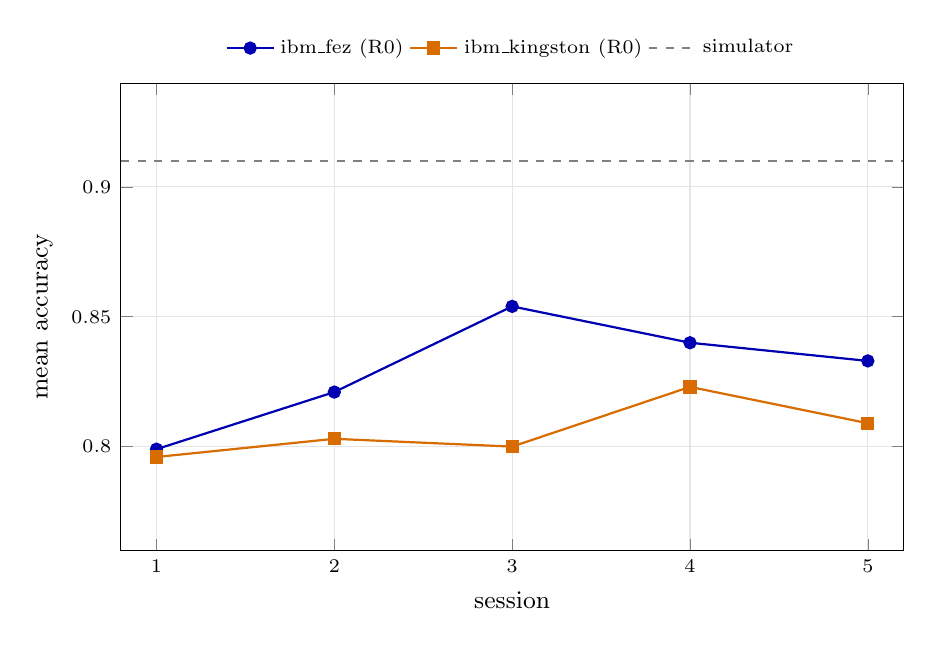
\begin{tikzpicture}
\begin{axis}[
  width=0.95\columnwidth, height=0.62\columnwidth,
  xmin=0.8, xmax=5.2, ymin=0.76, ymax=0.94, xtick={1,2,3,4,5},
  xlabel={session}, ylabel={mean accuracy},
  tick label style={font=\scriptsize}, label style={font=\small},
  legend columns=3, legend style={font=\scriptsize, draw=none, at={(0.5,1.03)}, anchor=south},
  grid=major, grid style={gray!20}]
\addplot[thick, mark=*, color=blue!70!black] coordinates
  {(1,0.799) (2,0.821) (3,0.854) (4,0.840) (5,0.833)};
\addlegendentry{ibm\_fez (R0)}
\addplot[thick, mark=square*, color=orange!85!black] coordinates
  {(1,0.796) (2,0.803) (3,0.800) (4,0.823) (5,0.809)};
\addlegendentry{ibm\_kingston (R0)}
\addplot[dashed, thick, gray] coordinates {(0.8,0.910) (5.2,0.910)};
\addlegendentry{simulator}
\end{axis}
\end{tikzpicture}
\caption{Hardware accuracy without repair in each session, averaged over datasets and models. The
dashed line is the simulator. Both devices stay well below it and move from session to session.}
\label{fig:drift}
\end{figure}

In the registered regression the CZ error, and not the readout error, had the largest coefficient (0.0151 per
standard deviation) and readout error came second (0.0110), so H4 is not supported. This result depends on a small number of inputs. In session 3 on \texttt{ibm\_kingston}, IBM's own
calibration marked two couplers inside our fixed chains as not working, and the job ran on them
anyway. In an exploratory check that was not part of the registration, we refitted the model without
these 132 observations. The readout error then becomes the largest term (0.0112) and the CZ error
falls to 0.0037. The registered decision on H4 is unchanged, but it rests on these inputs. Chains with a longer $T_2$ also had smaller errors.

\subsection{Noise model on Heron (RQ3)}
A straight line $\phi_{\mathrm{hw}}\approx\gamma\,\phi_{\mathrm{sim}}+\beta$, fitted for each
feature and session, described the hardware features well, with a median $R^2$ of 0.912. The noise therefore acts mainly as a contraction of the features toward zero. The median scale was $\gamma=0.922$ and
the median shift was 0.009. The scale differed a little between models (0.895 for M1, 0.953
for M2 and 0.889 for M3) but barely moved between sessions, with a typical spread of 0.026. So the
scale and shift picture from QuantumNAT \cite{wang2022quantumnat} holds on Heron and is stable over the campaign. However, as shown below, correcting this
contraction does not restore the accuracy.

\subsection{Repairs and their cost (RQ4)}
The repairs recovered little of the gap (Table~\ref{tab:repairs} and Fig.~\ref{fig:repairs}); the
best recovered 15\% of it. Two repairs had a gain whose
interval sat fully above zero. Measured readout correction (R3$_\mathrm{m}$) added 1.0 point for
1.06 seconds per session. The head trained on emulated noisy features (R4) added 0.8 points at no QPU cost. Refitting on 16 hardware labels (R2$_{16}$) added 0.3 points, but its interval starts at zero. Every other repair had an interval that includes zero, normalisation (R1) and
readout correction from the published numbers (R3$_\mathrm{r}$) among them. Since R2$_{16}$ was not
clearly better than R1, H3 is not supported. R4 also produced the best calibrated probabilities, with
a calibration error of 0.092 against 0.121 without repair and 0.061 in the simulator.

\begin{table}[t]
\centering
\caption{Repairs ranked by accuracy gain over R0 in points, with a 95\% interval over 60 cases.
Gap is the share of the simulator to hardware gap that was won back. QPU is the extra time per
session.}
\label{tab:repairs}
\footnotesize
\setlength{\tabcolsep}{4pt}
\begin{tabular}{lcccr}
\toprule
Repair & Gain & Interval & Gap (\%) & QPU (s) \\
\midrule
R3$_{\mathrm{m}}$ & $+1.0$ & $+0.6$ to $+1.5$ & 15 & 1.06 \\
R4 & $+0.8$ & $+0.2$ to $+1.5$ & 6 & 0.00 \\
R2$_{16}$ & $+0.3$ & $0.0$ to $+0.7$ & 3 & 0.25 \\
R2$_{16}^{\mathrm{s1}}$ & $+0.3$ & $-0.1$ to $+0.7$ & 5 & 0.05 \\
R2$_{8}$ & $+0.1$ & $-0.3$ to $+0.4$ & 0 & 0.13 \\
R1 & $-0.1$ & $-0.6$ to $+0.5$ & $-2$ & 0.00 \\
R3$_{\mathrm{r}}$ & $-0.1$ & $-0.7$ to $+0.5$ & $-3$ & 0.00 \\
R2$_{32}$ & $-0.2$ & $-0.5$ to $+0.1$ & 1 & 0.50 \\
\bottomrule
\end{tabular}
\end{table}

\begin{figure}[t]
\centering
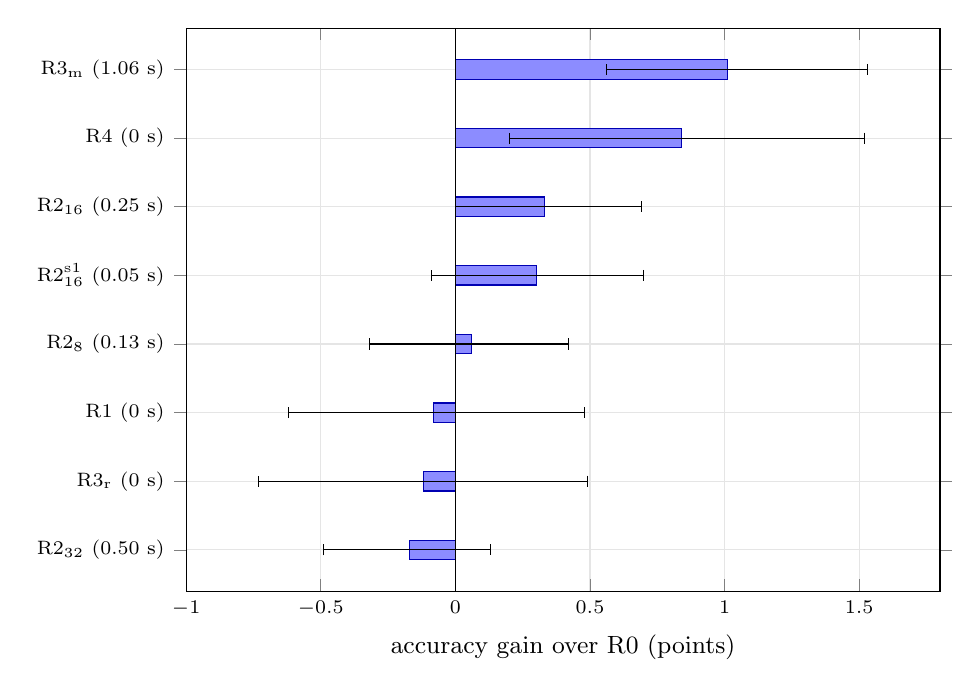
\begin{tikzpicture}
\begin{axis}[
  xbar, width=0.92\columnwidth, height=0.72\columnwidth,
  xmin=-1.0, xmax=1.8, ymin=0.4, ymax=8.6,
  ytick={1,2,3,4,5,6,7,8},
  yticklabels={R2$_{32}$ (0.50 s), R3$_\mathrm{r}$ (0 s), R1 (0 s), R2$_{8}$ (0.13 s),
    R2$_{16}^{\mathrm{s1}}$ (0.05 s), R2$_{16}$ (0.25 s), R4 (0 s), R3$_\mathrm{m}$ (1.06 s)},
  xlabel={accuracy gain over R0 (points)},
  tick label style={font=\scriptsize}, label style={font=\small},
  bar width=7pt, grid=major, grid style={gray!20}]
\addplot[fill=blue!45, draw=blue!70!black,
  error bars/.cd, x dir=both, x explicit, error bar style={black}] coordinates {
  (-0.17,1) += (0.30,0) -= (0.32,0)
  (-0.12,2) += (0.61,0) -= (0.61,0)
  (-0.08,3) += (0.56,0) -= (0.54,0)
  (0.06,4) += (0.36,0) -= (0.38,0)
  (0.30,5) += (0.40,0) -= (0.39,0)
  (0.33,6) += (0.36,0) -= (0.33,0)
  (0.84,7) += (0.68,0) -= (0.64,0)
  (1.01,8) += (0.52,0) -= (0.45,0)};
\draw[black] (axis cs:0,0.4) -- (axis cs:0,8.6);
\end{axis}
\end{tikzpicture}
\caption{Mean accuracy gain of each repair with its 95\% interval. The extra QPU seconds per
session are shown next to each name. Only R3$_\mathrm{m}$ and R4 are clearly above zero.}
\label{fig:repairs}
\end{figure}

Prediction sets calibrated on simulator data
covered the true label too rarely on hardware (Table~\ref{tab:coverage} and
Fig.~\ref{fig:coverage}). Their mean coverage was 0.849 and fell to 0.693 in the worst session and
model, against a nominal coverage of 0.90. Calibration on hardware data removed this undercoverage. Sets calibrated on the session 1 pool covered 0.944 of labels over all sessions and 0.948 in
sessions 2 to 5, and sets calibrated in the same session covered 0.929. Both exceed the nominal
level. The registered rule for H5 required the upper bound of the CP$_\mathrm{s1}$ coverage in
sessions 2 to 5 to fall below 0.90 and the mean ACI coverage to lie within 0.03 of 0.90. The ACI
condition was met (0.903), but the CP$_\mathrm{s1}$ interval was 0.937 to 0.958, entirely above
the nominal level, so H5 is not supported. Over these 16 days the drift was therefore not large enough to invalidate a hardware
calibration. ACI stayed close to the nominal level, at 0.901 on average and 0.880 at worst, with smaller sets (1.25 labels)
than the two hardware calibrated methods. It needs no extra QPU time, but it does assume that the
true label of each input becomes known after the prediction.

\begin{table}[t]
\centering
\caption{Prediction sets on hardware with a nominal coverage of 0.90. Coverage is averaged over all
sessions and over sessions 2 to 5 only, the window used by H5. Min is the worst session and model.
Size is the mean number of labels in a set.}
\label{tab:coverage}
\footnotesize
\setlength{\tabcolsep}{4pt}
\begin{tabular}{lccccr}
\toprule
Method & All & Sessions 2 to 5 & Min & Size & QPU (s) \\
\midrule
CP$_{\mathrm{sim}}$ & 0.849 & 0.856 & 0.693 & 1.08 & 0.00 \\
CP$_{\mathrm{s1}}$ & 0.944 & 0.948 & 0.860 & 1.45 & 0.10 \\
CP$_{\mathrm{same}}$ & 0.929 & 0.929 & 0.793 & 1.37 & 0.50 \\
ACI & 0.901 & 0.903 & 0.880 & 1.25 & 0.00 \\
\bottomrule
\end{tabular}
\end{table}

\begin{figure}[t]
\centering
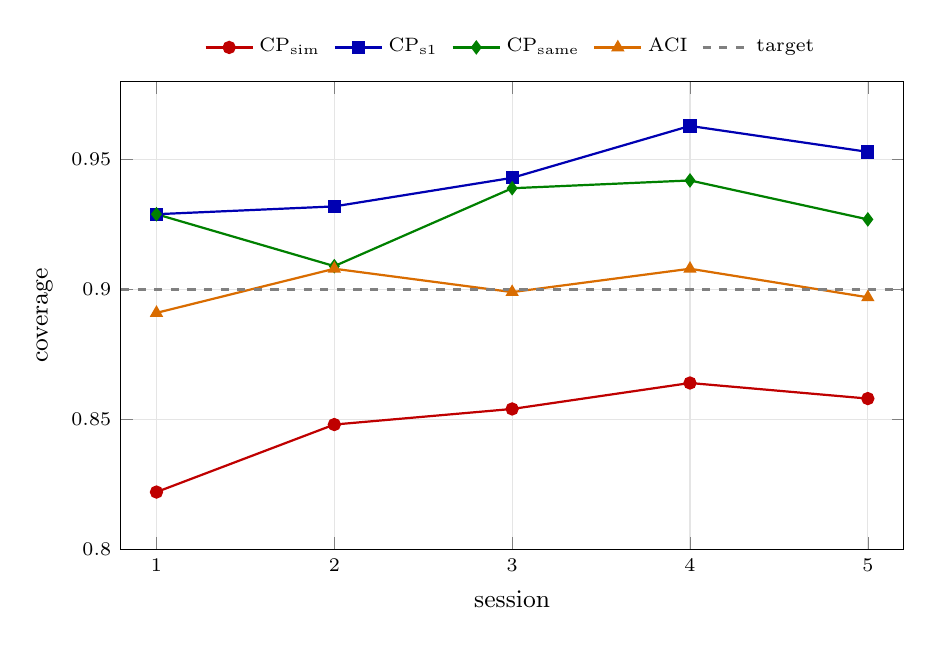
\begin{tikzpicture}
\begin{axis}[
  width=0.95\columnwidth, height=0.62\columnwidth,
  xmin=0.8, xmax=5.2, ymin=0.80, ymax=0.98, xtick={1,2,3,4,5},
  xlabel={session}, ylabel={coverage},
  tick label style={font=\scriptsize}, label style={font=\small},
  legend columns=5,
  legend style={font=\scriptsize, draw=none, at={(0.5,1.03)}, anchor=south, /tikz/every even column/.append style={column sep=3pt}},
  grid=major, grid style={gray!20}]
\addplot[thick, mark=*, color=red!75!black] coordinates
  {(1,0.822) (2,0.848) (3,0.854) (4,0.864) (5,0.858)};
\addlegendentry{CP$_\mathrm{sim}$}
\addplot[thick, mark=square*, color=blue!70!black] coordinates
  {(1,0.929) (2,0.932) (3,0.943) (4,0.963) (5,0.953)};
\addlegendentry{CP$_\mathrm{s1}$}
\addplot[thick, mark=diamond*, color=green!50!black] coordinates
  {(1,0.929) (2,0.909) (3,0.939) (4,0.942) (5,0.927)};
\addlegendentry{CP$_\mathrm{same}$}
\addplot[thick, mark=triangle*, color=orange!85!black] coordinates
  {(1,0.891) (2,0.908) (3,0.899) (4,0.908) (5,0.897)};
\addlegendentry{ACI}
\addplot[dashed, gray, thick] coordinates {(0.8,0.90) (5.2,0.90)};
\addlegendentry{target}
\end{axis}
\end{tikzpicture}
\caption{Coverage of the prediction sets in each session, averaged over devices, datasets and
models. Simulator calibration stays below the target in every session.}
\label{fig:coverage}
\end{figure}

\begin{table*}[t]
\centering
\caption{Registered hypotheses with the measured value and the decision.}
\label{tab:hypotheses}
\footnotesize
\renewcommand{\arraystretch}{1.15}
\begin{tabular}{lL{6.2cm}L{6.4cm}l}
\toprule
 & Hypothesis & Result (mean and 95\% interval) & Decision \\
\midrule
H1 & the emulator overestimates hardware accuracy & emulator minus hardware is 0.055 (0.042 to 0.069) & supported \\
H2 & variation across sessions is larger than shot noise & variance ratio is 3.80 (3.42 to 4.24) & supported \\
H3 & a refit on 16 labels beats normalisation & R2$_{16}$ minus R1 is 0.004 ($-$0.001 to 0.009) & not supported \\
H4 & readout error is the strongest calibration predictor & the largest term is the CZ error & not supported \\
H5 & sets calibrated in session 1 undercover later sessions while ACI holds & CP$_\mathrm{s1}$ covers 0.948 and ACI covers 0.903 & not supported \\
\bottomrule
\end{tabular}
\end{table*}

%======================================================================
\section{Discussion}

\subsection{Implications}
An emulator built from calibration data is useful for screening but does not replace hardware runs. In our data it ordered the configurations correctly in most cases while overstating their
accuracy by 5.5 points. The QAOA
study on Heron reported a similar overestimate \cite{qaoa2026drift}, which suggests that the effect is not specific
to classifiers. Drift between days was present on both devices and was not only a degradation, since both
processors moved toward the simulator over the campaign. A single session can be several
points away from the average, so a result from one day of hardware should be checked on another
day. Here a repeat costs about 20 seconds of QPU time, a small cost for a check of temporal stability.

Under a free budget the low cost repairs gave small gains. Measured readout correction and the noise
aware head each added about a point, and the head needs no QPU time and also gives better calibrated probabilities. Normalisation, which helped a lot on older IBM devices
\cite{wang2022quantumnat}, gave no gain here. The global shrinkage of the features is small and
stable, which suggests that the remaining loss comes from errors that differ from input to input and from
chain to chain, and that a single global correction cannot remove. For uncertainty, calibration on hardware data
was sufficient: labels from any session restored coverage, and ACI held the target
with smaller sets.

\subsection{Limitations}
On the free plan a job runs when the queue lets it, and not at a chosen time. The models are small, with
four qubits and at most nine CZ gates, and with 150 test inputs per session only effects pooled
over sessions can be resolved. We chose the qubit chains from one day of calibration and then kept
them fixed. This pairs the data, but later sessions may not have used the best qubits of
their day, and the layout could not react when two couplers failed. Checking the fixed chains against the current calibration before each job would detect such
cases. The emulator has no
crosstalk and our pilot can only rule out large crosstalk. Finally, twirling and dynamical decoupling were disabled by design, so our numbers describe raw device noise.

\subsection{Changes from the registered plan}
Before the hypotheses were first tested we found and fixed one bug in the analysis code.
Calibration age had been measured at download time instead of job start, which only affects one
term of the H4 regression. The plan asked for sessions at a similar time of day, but the queue and our schedules did not always allow this. Session 2 on both devices ran close to midnight India
time, and in total four sessions started in the day and six at night. The campaign stretched over
16.5 days, 2.5 days past the planned maximum of 14. On \texttt{ibm\_kingston}, session 5 started
only 2.9 hours after session 4, at 01:34 India time. Leaving out such close pairs, again as an exploratory check that was not registered, lowers the
variance ratio from 3.80 to 3.40 (interval 3.08 to 3.76), so the drift result holds.

%======================================================================
\section{Conclusion}
We followed simulator trained quantum classifiers on two IBM Heron processors for 16 days, using a
registered plan that fits inside a free account. Across this campaign the calibration emulator overestimated hardware accuracy, and the variation
between sessions exceeded shot noise on both devices. The low cost repairs we tested recovered only
a small part of the accuracy gap. Prediction sets were the exception, since calibrating them on
hardware data, or updating them online, restored the nominal coverage. Our results therefore
favour repeating hardware runs on more than one day and calibrating uncertainty on hardware data
rather than in simulation. Where accuracy has to be recovered under a tight budget, repairs that
need little or no QPU time, such as the noise aware head, are the most practical choice. Future work should include more devices, longer campaigns, larger models and runs with twirling and dynamical
decoupling switched on.

\section*{Data and code availability}
The code, frozen models, raw counts and calibration snapshots are available at
\url{https://github.com/pankajbaid567/QML-research}. The registered plan is the git tag
\texttt{prereg-v1} (commit \texttt{154984c} on 27 October 2026).

\section*{Use of AI tools}
We want to be open about how this paper was made. AI assistants (Kiro and Claude) were used to help
write the analysis software and to draft and edit the text of this paper, including this simplified
and final version. The hardware jobs were run from the authors' own IBM Quantum accounts. Every
number in the paper is produced by the analysis code from the raw data in the repository above, so
anyone can check it. The authors reviewed the manuscript and take full responsibility for its
content.

\section*{Acknowledgment}
We acknowledge the use of IBM Quantum services for this work. The views expressed are those of
the authors, and do not reflect the official policy or position of IBM or the IBM Quantum team.

%======================================================================
\begin{thebibliography}{99}

\bibitem{wang2021nibp}
S. Wang, E. Fontana, M. Cerezo, K. Sharma, A. Sone, L. Cincio, and P. J. Coles, ``Noise-induced
barren plateaus in variational quantum algorithms,'' \emph{Nature Communications}, vol. 12,
p. 6961, 2021.

\bibitem{heyraud2022noisykernels}
V. Heyraud, Z. Li, Z. Denis, A. Le Boit\'e, and C. Ciuti, ``Noisy quantum kernel machines,''
\emph{Physical Review A}, vol. 106, p. 052421, 2022.

\bibitem{realtimecal2023}
Y. Liu, Z. Li, A. Robertson, X. Fu, and S. L. Song, ``Enabling efficient real-time calibration on
cloud quantum machines,'' \emph{IEEE Transactions on Quantum Engineering}, vol. 4, pp. 1--17,
2023.

\bibitem{wang2022quantumnat}
H. Wang, J. Gu, Y. Ding, Z. Li, F. T. Chong, D. Z. Pan, and S. Han, ``QuantumNAT: Quantum
noise-aware training with noise injection, quantization and normalization,'' in \emph{Proc. 59th
ACM/IEEE Design Automation Conference (DAC)}, 2022.

\bibitem{nation2021m3}
P. D. Nation, H. Kang, N. Sundaresan, and J. M. Gambetta, ``Scalable mitigation of measurement
errors on quantum computers,'' \emph{PRX Quantum}, vol. 2, p. 040326, 2021.

\bibitem{vandenberg2022trex}
E. van den Berg, Z. K. Minev, and K. Temme, ``Model-free readout-error mitigation for quantum
expectation values,'' \emph{Physical Review A}, vol. 105, p. 032620, 2022.

\bibitem{park2023qcp}
S. Park and O. Simeone, ``Quantum conformal prediction for reliable uncertainty quantification in
quantum machine learning,'' \emph{IEEE Transactions on Quantum Engineering}, 2023.

\bibitem{spencer2026aqcp}
D. Spencer, S. Nicholls, and M. Caprio, ``Adaptive conformal prediction for quantum machine
learning,'' \emph{Transactions on Machine Learning Research}, 2026, arXiv:2511.18225.

\bibitem{qaoa2026drift}
A. Vishwakarma, ``When does calibration-aware compilation transfer to quantum hardware? A
three-processor QAOA study of ranking, drift, and refresh,'' \emph{Quantum Science and
Technology}, 2026, doi:10.1088/2058-9565/aeb8eb.

\bibitem{bowles2024benchmarking}
J. Bowles, S. Ahmed, and M. Schuld, ``Better than classical? The subtle art of benchmarking
quantum machine learning models,'' arXiv:2403.07059, 2024.

\bibitem{schuld2022advantage}
M. Schuld and N. Killoran, ``Is quantum advantage the right goal for quantum machine learning?''
\emph{PRX Quantum}, vol. 3, p. 030101, 2022.

\bibitem{havlicek2019supervised}
V. Havl\'i\v{c}ek, A. D. C\'orcoles, K. Temme, A. W. Harrow, A. Kandala, J. M. Chow, and
J. M. Gambetta, ``Supervised learning with quantum-enhanced feature spaces,'' \emph{Nature},
vol. 567, pp. 209--212, 2019.

\bibitem{perezsalinas2020reuploading}
A. P\'erez-Salinas, A. Cervera-Lierta, E. Gil-Fuster, and J. I. Latorre, ``Data re-uploading for a
universal quantum classifier,'' \emph{Quantum}, vol. 4, p. 226, 2020.

\bibitem{huang2021power}
H.-Y. Huang, M. Broughton, M. Mohseni, R. Babbush, S. Boixo, H. Neven, and J. R. McClean, ``Power
of data in quantum machine learning,'' \emph{Nature Communications}, vol. 12, p. 2631, 2021.

\bibitem{yasuda2023qrc}
T. Yasuda \emph{et al.}, ``Quantum reservoir computing with repeated measurements on
superconducting devices,'' arXiv:2310.06706, 2023.

\bibitem{thanasilp2024concentration}
S. Thanasilp, S. Wang, M. Cerezo, and Z. Holmes, ``Exponential concentration in quantum kernel
methods,'' \emph{Nature Communications}, vol. 15, p. 5200, 2024.

\bibitem{wang2022quantumnas}
H. Wang, Y. Ding, J. Gu, Y. Lin, D. Z. Pan, F. T. Chong, and S. Han, ``QuantumNAS: Noise-adaptive
search for robust quantum circuits,'' in \emph{Proc. IEEE International Symposium on
High-Performance Computer Architecture (HPCA)}, 2022.

\bibitem{temme2017zne}
K. Temme, S. Bravyi, and J. M. Gambetta, ``Error mitigation for short-depth quantum circuits,''
\emph{Physical Review Letters}, vol. 119, p. 180509, 2017.

\bibitem{liao2024mlqem}
H. Liao, D. S. Wang, I. Sitdikov, C. Salcedo, A. Seif, and Z. K. Minev, ``Machine learning for
practical quantum error mitigation,'' \emph{Nature Machine Intelligence}, 2024.

\bibitem{guo2017calibration}
C. Guo, G. Pleiss, Y. Sun, and K. Q. Weinberger, ``On calibration of modern neural networks,'' in
\emph{Proc. 34th International Conference on Machine Learning (ICML)}, 2017.

\bibitem{gibbs2021aci}
I. Gibbs and E. Cand\`es, ``Adaptive conformal inference under distribution shift,'' in
\emph{Advances in Neural Information Processing Systems (NeurIPS)}, 2021.

\bibitem{qbiobench2026}
M. Sokol, J. Hejda, P. Volf, and P. Kut\'ilek, ``QBioBench: Benchmark of quantum machine learning
for peripheral biosignals on real hardware,'' \emph{Quantum Science and Technology}, 2026,
doi:10.1088/2058-9565/aeb71e.

\bibitem{farib2026crossdevice}
S. A. Farib, S. R. Islam, and A. R. Anik, ``Few-shot cross-device transfer for quantum noise
modeling on real hardware,'' arXiv:2604.24397, 2026.

\bibitem{murali2020crosstalk}
P. Murali, D. C. McKay, M. Martonosi, and A. Javadi-Abhari, ``Software mitigation of crosstalk on
noisy intermediate-scale quantum computers,'' in \emph{Proc. ASPLOS}, 2020.

\bibitem{ohkura2022simultaneous}
Y. Ohkura, T. Satoh, and R. Van Meter, ``Simultaneous execution of quantum circuits on current and
near-future NISQ systems,'' \emph{IEEE Transactions on Quantum Engineering}, vol. 3, 2022.

\bibitem{wolberg1993breast}
W. Wolberg, O. Mangasarian, N. Street, and W. Street, ``Breast cancer Wisconsin (diagnostic),''
UCI Machine Learning Repository, 1993.

\bibitem{javadiabhari2024qiskit}
A. Javadi-Abhari \emph{et al.}, ``Quantum computing with Qiskit,'' arXiv:2405.08810, 2024.

\end{thebibliography}

\end{document}
